\ifdefined\USERMANUAL
  \newcommand{\doctype}{ユーザーマニュアル}
\else
  \newcommand{\doctype}{リファレンスカード}
\fi

\maketitlepage{TAIPO}{MIDIエクステンダー}{TAIPO_SILVER_cutout_small_2}{\doctype}

\newpage
\tableofcontents
\newpage
\part{概要}
\newpage
\section{概要}\label{section:installation}
\subsection{概要}
\paragraph*{}
\textbf{TAIPO} MIDIエクステンダーは、標準MIDI TRSタイプBケーブルを使用して、The Centreを外部機器(コンピュータを含む)にシームレスに接続します。
\subsection{同梱物}
\paragraph*{}
\textbf{TAIPO}のパッケージには以下の付属品が含まれています:
\begin{enumerate}
  \item \textbf{TAIPO} Eurorackモジュール
  \item 標準Eurorack電源ケーブル(10ピンから16ピン)
  \item \textbf{The Centre}との接続用のMIDI-EXリンクケーブル
\end{enumerate}

\newpage
\part{インストール}
\newpage
\section{インストール}
\subsection{インストール手順}
\paragraph*{}
\textbf{TAIPO}モジュールのインストールは、ユーザーのケースにEurorackモジュールをインストールする標準手順に従います。

\begin{figure}[h]
  \centering
  \includegraphics[height=0.5\linewidth]{taipo_the_centre_cable_install.jpg}
  \includegraphics[height=0.5\linewidth]{taipo_cable_install.jpg}
  \caption{両端のケーブル設置}
  \label{fig:midsinglenote}
\end{figure}

\subsection{重要なインストール上の注意}
\paragraph*{}
インストール時にはケーブルの向きを正しくしてください。The Centre側の色の順序は上から\textbf{黒、赤、黄、緑}であるべきで、TAIPO側では逆の\textbf{緑、黄、赤、黒}となります。
\newline$\blacksquare$ \textbf{重要}:The Centre側では、上図に示されているようにMIDI-EXコネクタに接続してください。2番目のコネクタはThe CentreのMIDI出力をTWINSに接続するために使用されます。

\newpage
\part{MIDI}
\newpage
\section{MIDIケーブルの種類}
\subsection{TAIPOケーブルの種類}
\paragraph*{}
\textbf{TAIPO}は3.5mm TRS(チップ-リング-シールド)タイプBケーブルを使用します。詳細は\underline{\nameref{section:cabletypeb}}を参照してください。
\subsection{MIDI信号について}
\paragraph*{}
MIDI信号は、MIDIケーブルを介してRS-232プロトコルを使用して、非標準の31,250ボー(毎秒ビット数)で送信されます。MIDI接続は方向性があり、ケーブル内のピンの内部構成が重要です。これは電流が一方向に流れるためです。標準MIDI DINケーブルでは問題ありませんが、3.5mm TRSケーブルは当初統一規格がなかったため、異なる配線方式が生じ、複数の規格が登場しました。
\newline$\blacksquare$ \textbf{注意}:異なるTRS規格は互換性がなく、交換もできません。異なるTRS規格のデバイスを接続するには、適合したケーブルを使用する必要があります。
\subsection{DINコネクタ}
標準MIDIケーブルは、信頼性の高い接続を確保するために5ピンのDINコネクタを使用します。
\subsection{TRSコネクタの種類}
\subsubsection{タイプAコネクタ}
TRSタイプAは、3.5mmジャックの\textbf{チップ}を\textit{\textbf{ソース}}、\textbf{リング}を\textit{\textbf{シンク}}と定義します。
\newline
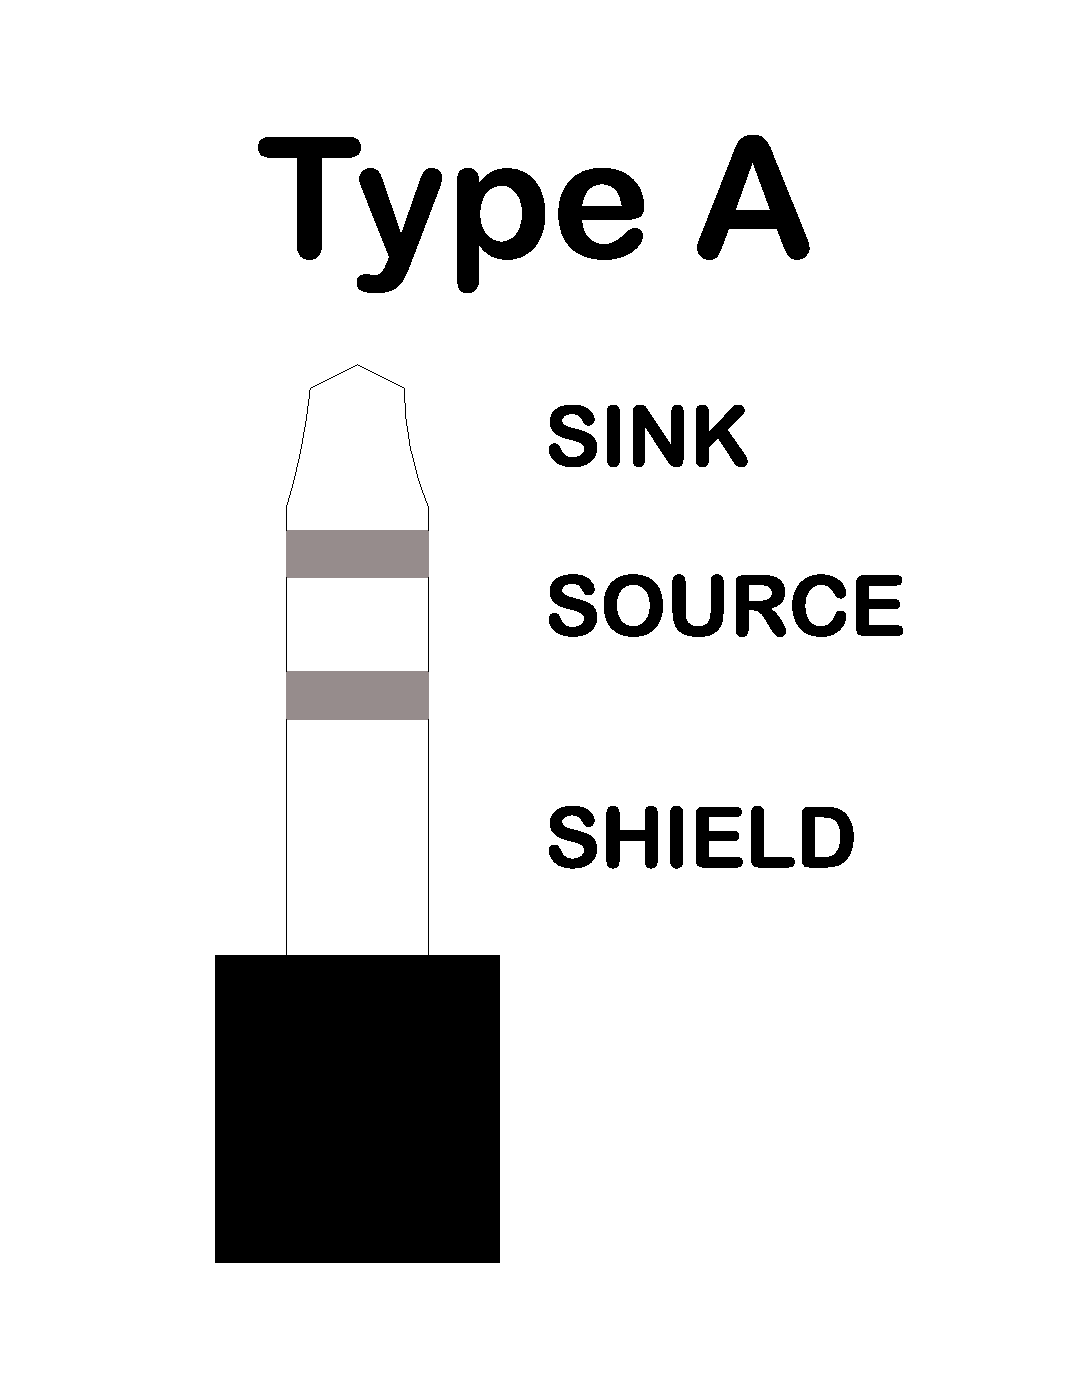
\includegraphics[height=0.3\linewidth]{midi_trs_type_a.eps}
\newline$\bigstar$ タイプAを使用するブランド:Korg、Akai
\subsubsection{タイプBコネクタ}\label{section:cabletypeb}
TRSタイプBは、3.5mmジャックの\textbf{チップ}を\textit{\textbf{シンク}}、\textbf{リング}を\textit{\textbf{ソース}}と定義します。
\newline$\blacksquare$ タイプBはEurorackモジュラーコミュニティで広く使用されています。
\newline
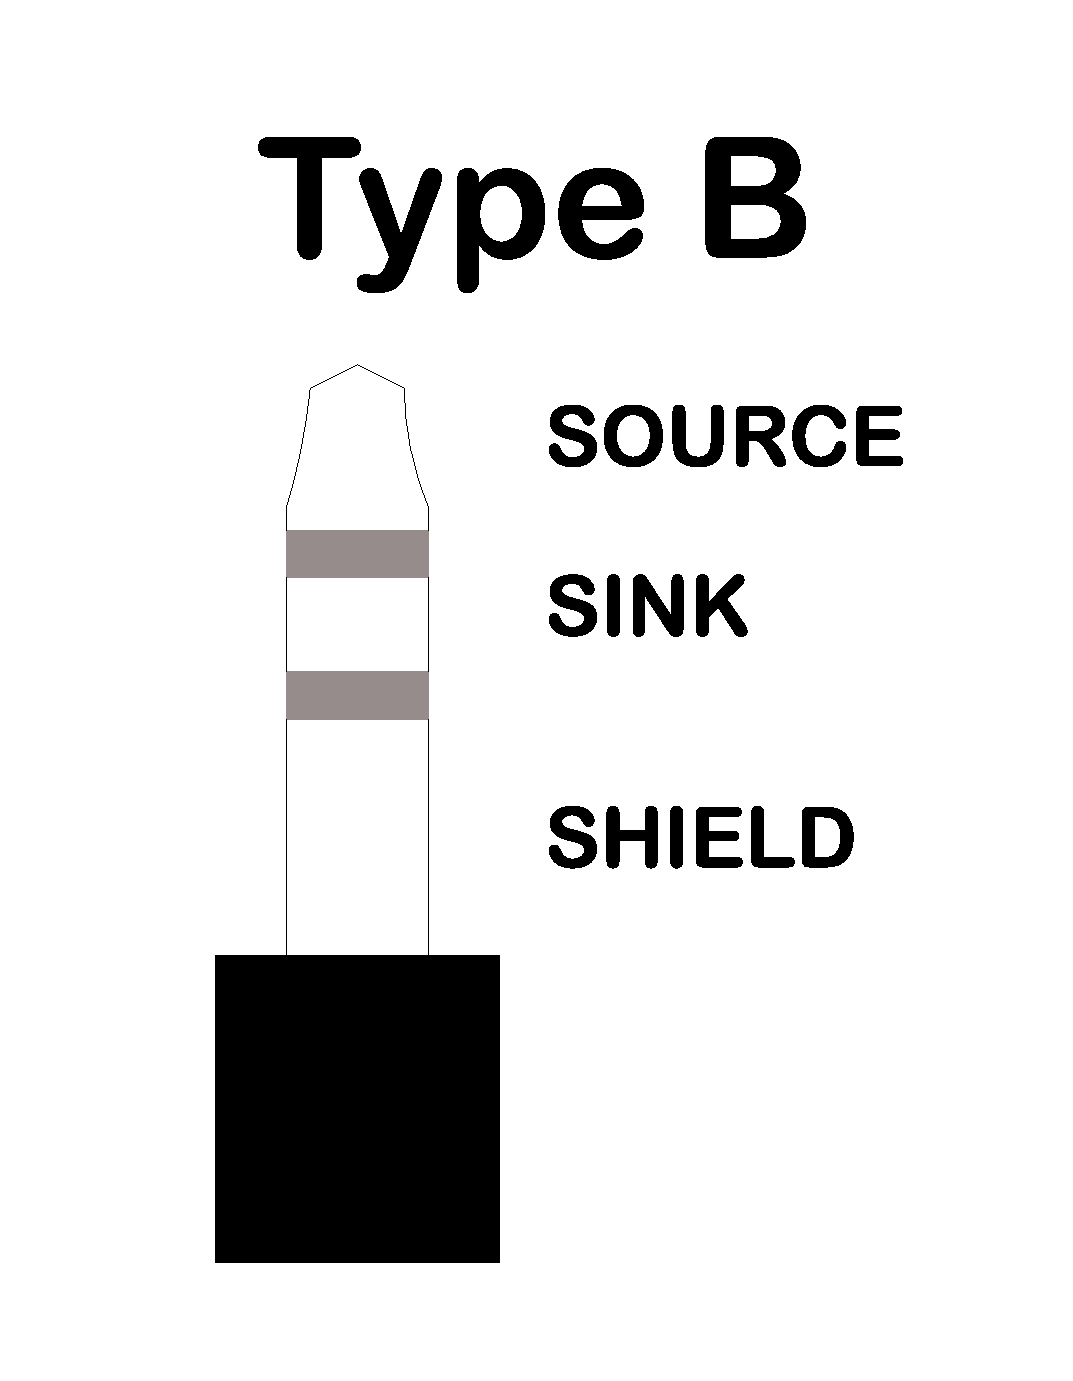
\includegraphics[height=0.3\linewidth]{midi_trs_type_b.eps}
\newline$\bigstar$ タイプBを使用するブランド:Arturia、Novation、1010 Music